\section{Other Results}

\subsection{$k$-nary trees}
\begin{lemma}The depth of a complete $k$-nary tree $d$ values $\left\lfloor\log_k((k-1)n)\right\rfloor$
\end{lemma}
\begin{proof}
	\begin{align}
		n &= \sum_{i=0}^{d}k^i = \frac{k^{d+1}-1}{k-1}\\
		\Leftrightarrow d &= \log_k((k-1)n+1)-1 = \left\lfloor\log_k((k-1)n)\right\rfloor
	\end{align}
\end{proof}

\begin{theorem}
	Every $k$-nary tree admits a polyline drawing with a nearly optimal ratio, apart from a rounding error $\varepsilon$ on area $\mathcal{O}(n^2\log n)$, allowing one bend per edge.
\end{theorem}
\begin{proof}
	Generally, the reulting drawing will be constructed from top to bottom. The root vertex lies on top, the leaves lie on the bottom. Let $l := k^d +1$. From the root vertex, place one vertex $k^d $ \UL~to the left and one unit down. Place another child $k^d$ \UL~to the right and one unit down. For the remaining $k-2$ children, place bends inbetween those outer children equidistantly. Connect the two children and the bend points with the root with a line segment. There, the rounding error takes effect and is bound by $1$. Place the remaining children below the respective bends so that the sum of the line segment equals $l$, apart from the rounding error. Between two children, there are $\frac{2k^d}{k-1}-2$ free columns for the remaining drawing.\\
	Further iterate over the depth. For depth $i$, place the outermost children $k^{d-(i-1)}$ aside and one unit down and the $k-2$ bend points in between equidistantly. From the preceding depth, there are $\frac{2k^{d-(i-2)}}{k-1}-2$ free columns between two children of depth $i$ placed next to each other. Since $\frac{k^{d-(i-1)}}{k-1}\leq \frac{k^{d-(i-2)}}{k-1}$, the area for depth $i+1$ is guaranteed.\\
	The total width of the drawing is bound by $2\cdot \sum_{i=0}^{d}k^i \in \mathcal{O}(n)$, and the total height is bound by $d\cdot l = d\cdot (k^d+1) \in \mathcal{O}(n \log n)$. Every edge has length of approximately $l$, apart from a rounding error derived by the diagonals with one bend per edge and the total area consumption values $\mathcal{O}(n^2\log n)$.
\end{proof}
\begin{figure}[H]
	\centering
	\begin{subfigure}{0.8\linewidth}
		\centering
		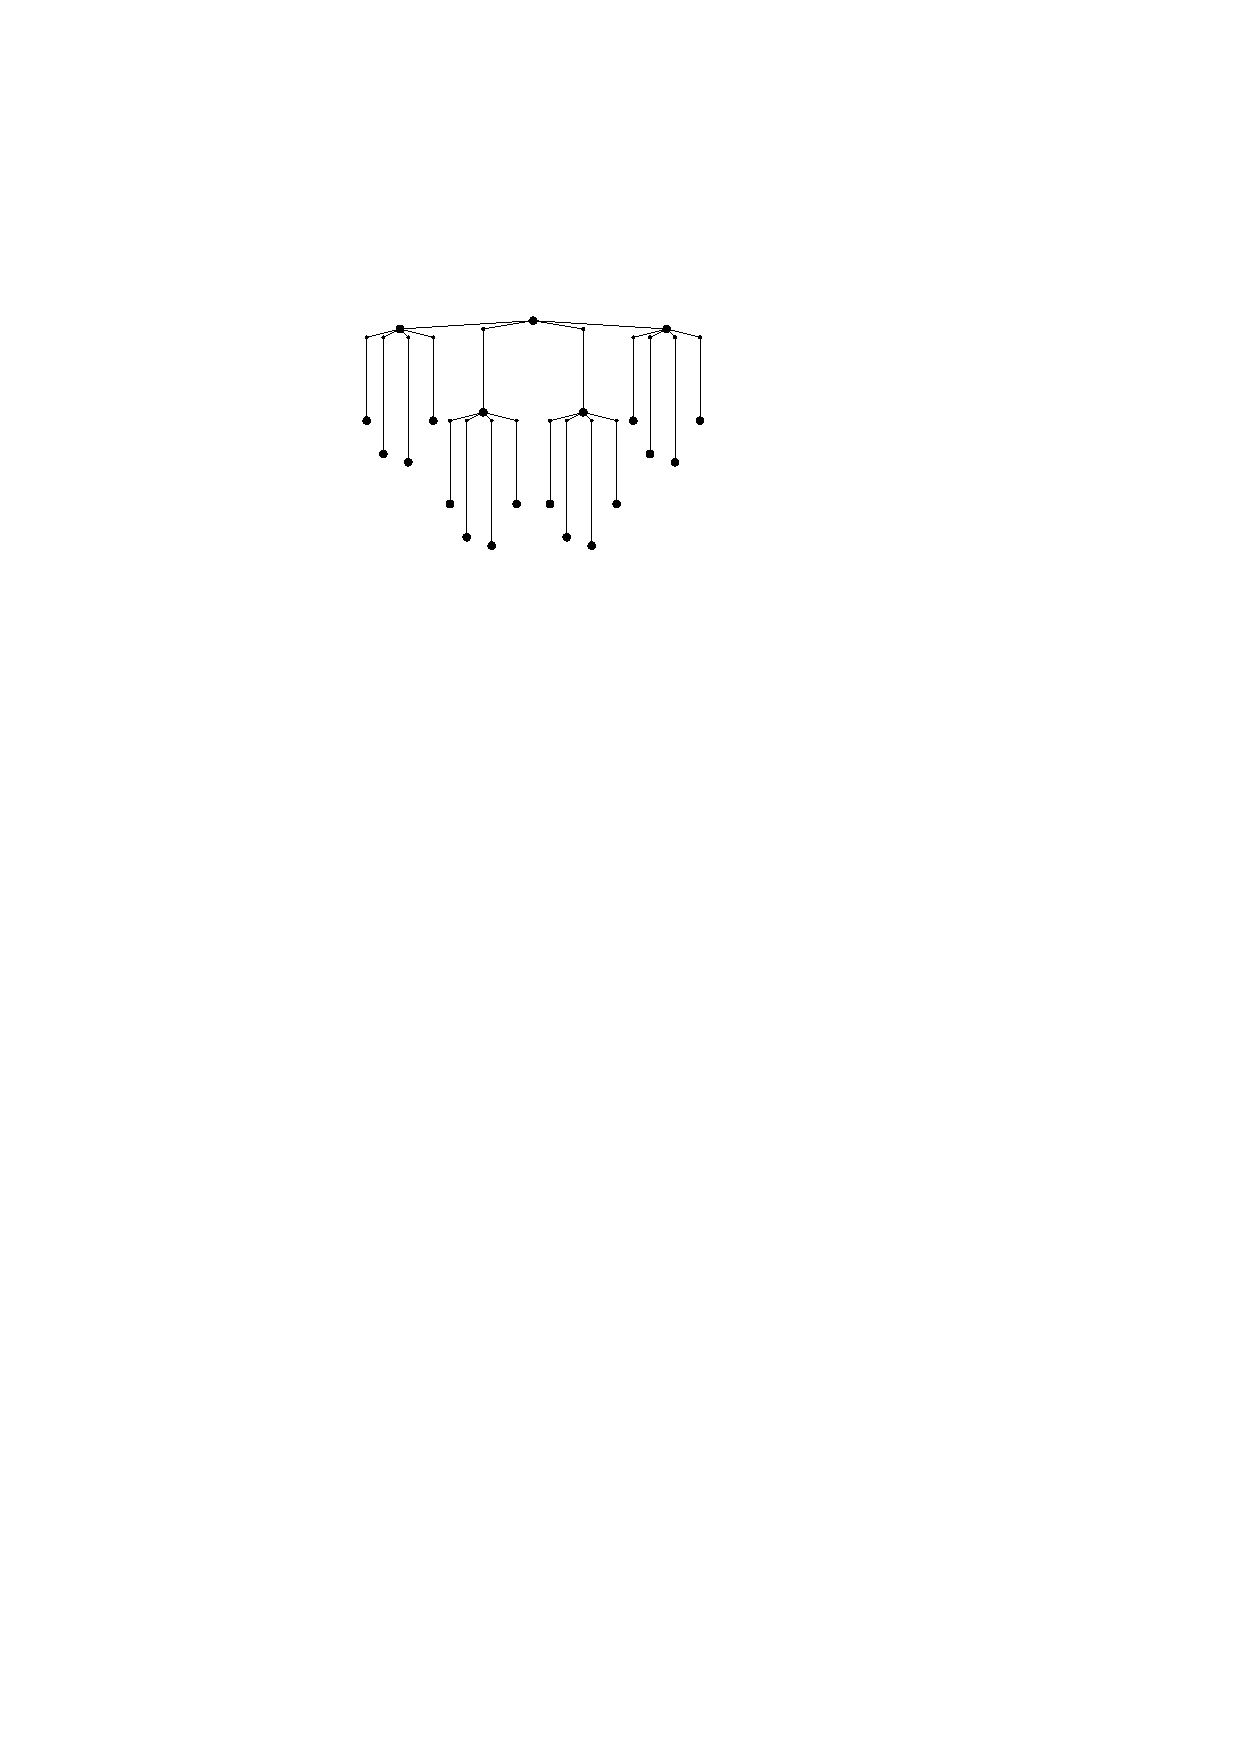
\includegraphics[width=\textwidth,page=1]{drawings/4-ary_tree.pdf}
	\end{subfigure}
	\caption{Complete 4-ary tree with depth 2}\label{im:4-ary_d=2}
\end{figure}
\begin{figure}[H]
	\centering
	\begin{subfigure}{0.8\linewidth}
		\centering
		\includegraphics[width=\textwidth,page=2]{drawings/4-ary_tree.pdf}
	\end{subfigure}
	\caption{Complete 3-ary tree with depth 3}\label{im:4-ary_d=2}
\end{figure}
\subsection{Certain family of 3-trees}\label{section:3-tree-family}
Recall a $k$-tree, recursively defined. A 3-tree starts with a $K_4$ and every vertex inserted is connected to exactly three neighbours, creating a 4-clique.
\begin{theorem}
	There exists a family of 3-trees which obtain a polyline drawing with a constant edge-length ratio, allowing one bend per edge on area $\mathcal{O}(n^2)$.
\end{theorem}
\begin{proof}
	Let $G$ be a graph consisting of $\frac{n}{3}$ socalled \grqq nested\grqq~triangles, meaning that every triangle either encloses or is enclosed by another triangle.  Let $t_1$ be the outermost triangle and $t_{i+1}$ inside $t_i,i=1,...,\frac{n}{3}$. The vertices defining $t_i$ are called $A_i,B_i,C_i$. For the orientation, $A_i$ will be on the bottom left corner, $B_i$ on the bottom right corner and $C_i$ on the top corner. The edges between the triangles are defined as:
	\begin{align}
		&(A_i,A_{i+1}),(A_i,B_{i+1}),(A_i,C_{i+1})\\
		&(B_i,B_{i+1})\\
		&(C_i,C_{i+1}),(C_i,B_{i+1})
	\end{align}
		\begin{figure}[H]
	\centering
	\begin{subfigure}{0.8\linewidth}
		\centering
		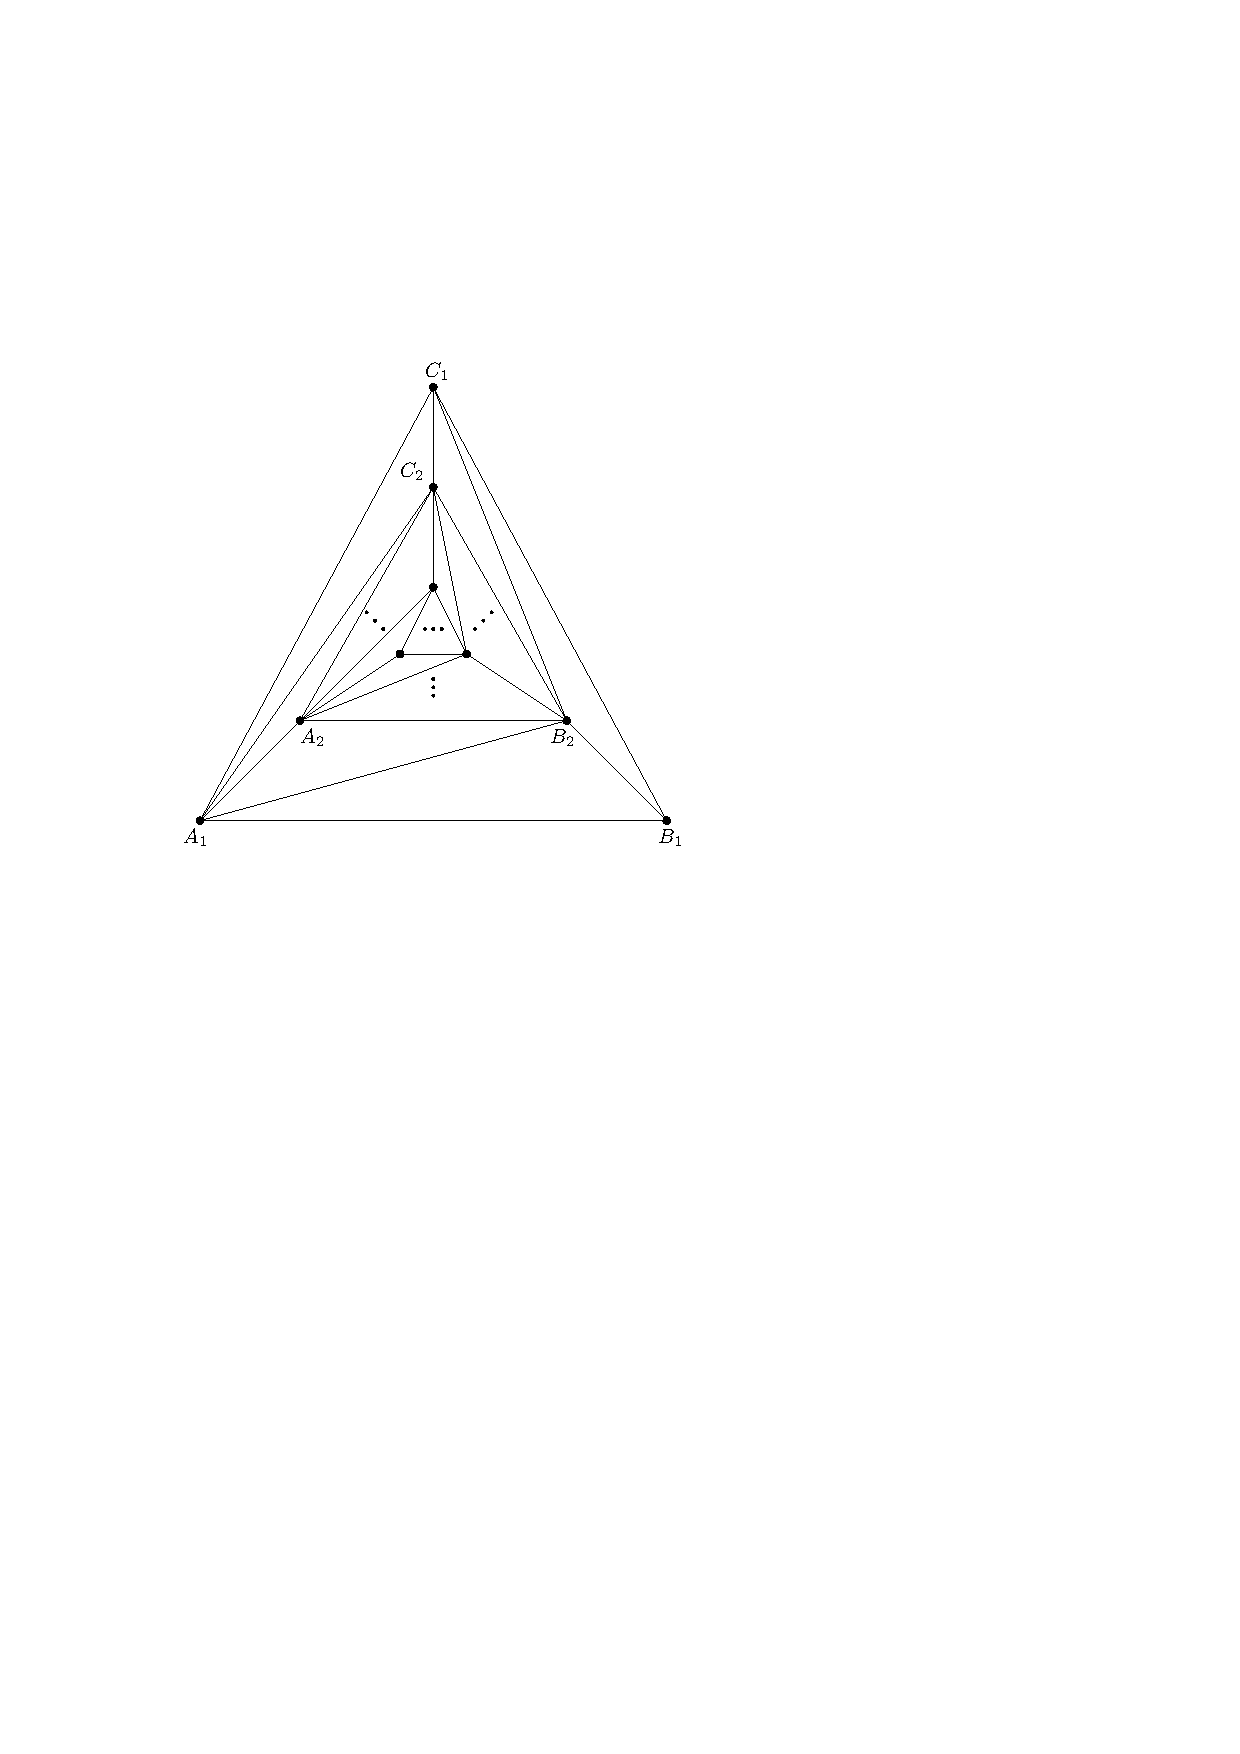
\includegraphics[width=\textwidth,page=1]{drawings/3-tree.pdf}
	\end{subfigure}
	\caption{3-tree with nested triangles}\label{im:3trees-straight-line}
\end{figure}
	The connections between the triangles $t_i,t_{i+1}$ fulfill the 3-tree property. (\cite{DBLP:journals/jgaa/MondalNRA11}, Lemma 12, Page 23).
	At first, draw the triangles with a spacing of three between two consecutive triangles. This ensures two rows or columns of availiable bend points inbetween. Placing bends will lengthen the connections between two successive triangles. The bend points are placed as illustrated in the following figure:
		\begin{figure}[H]
		\centering
		\begin{subfigure}{0.8\linewidth}
			\centering
			\includegraphics[width=\textwidth,page=2]{drawings/3-tree.pdf}
		\end{subfigure}
		\caption{Polyline drawing scheme with one bend per edge}\label{im:3trees-drawing}
	\end{figure}	
	Then, the length of every connecting edge between $t_i$ and $t_{i+1}$ is greater than the shortest edge of $t_{i+1}$. The total shortest edge lies in $t_{\frac{n}{3}}$. The total longest edge lies in $t_1$. Let the length of the edges of $t_{\frac{n}{3}}$ value $n$. Then, the length of the edges of $t_1$ value $n+2\cdot 3\left(\frac{n}{3}-1\right) = 3n-6$. The ratio is bound by 3, the spacing value. The output is a polyline drawing with one bend per edge on a grid of area $(3n-6)\times(3n-6)$.
\end{proof}
\subsection{Outerplanar graphs}
Outerplanar graphs are a family of series-parallel graphs. The result of 2-trees can be applied directly to outerplanar graphs. The following theorem describes the edge-length ratio in a poly-line drawing while maintaining that every vertex is placed on the outerface.
\begin{theorem}
	Every outerplanar graph $G$ obtains a poly-line drawing with an edge-length ratio of $\mathcal{O}(1)$ with up to four bends per edge in $\mathcal{O}(n^2)$ area.
\end{theorem}
\begin{proof}
	Since outerplanar graphs are series-parallel graphs, this proof is similar to the proof of Theorem \ref{theorem:2-tree_result}. By Biedl, it was proven, that only the base case, the parallel case and the serial case S1 and S2a take place (\cite{DBLP:journals/dcg/Biedl11}, Page 15). All the cases guarantee that the vertices lie on the outer face.
	\begin{figure}[H]
		\centering
		\begin{subfigure}{0.8\linewidth}
			\centering
			\includegraphics[width=0.8\textwidth,page=14]{drawings/2-trees.pdf}
		\end{subfigure}
		\caption{Case S2a is the only case for outerplanar graphs}\label{im:outerplanar}
	\end{figure}
	With the modification used in Theorem \ref{theorem:2-tree_result}, the height can be bound by:
	\begin{align}
		h_{mod}(m)\leq 3\log m + 2 + l_{\min} + 1\leq 3(\log 2 +1)+3\cdot \log n + n \in \mathcal{O}(n)
	\end{align}
	The longest edge can occur in case S2a, with two bends in the box drawing. In the polyline drawing, two additional bends are introduced for vertex $v,t$. Therefore, the longest edge is bound by:
	\begin{align}
		l_{\max}\leq 2(w_{mod}(m)+h_{mod}(m))= 6\cdot \log 2 +6\log n + 14n - 2
	\end{align}
	Then, it holds for the ratio:
	\begin{align}r \leq \frac{20n}{n} = 20 \in \mathcal{O}(1)
	\end{align}
\end{proof}